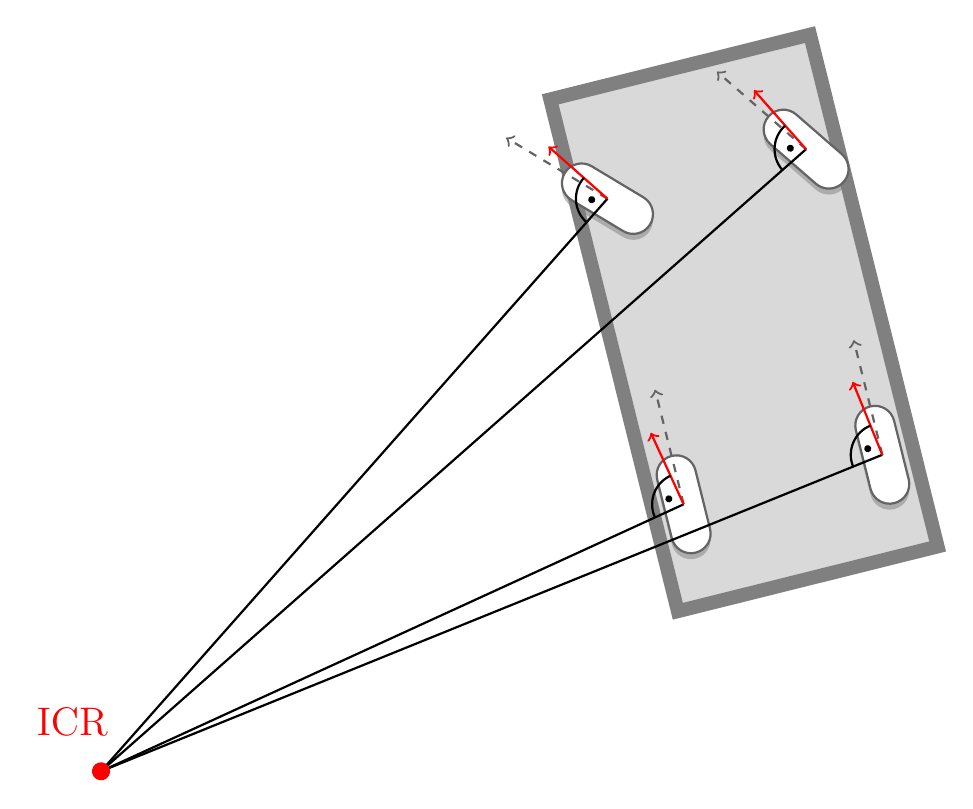
\begin{tikzpicture}[thick]
\usetikzlibrary{shapes.misc,shadows}
\usetikzlibrary{calc}
\usetikzlibrary{positioning,backgrounds}

\pgfmathsetmacro{\ArrowLength}{1}
\pgfmathsetmacro{\vheight}{4}
\pgfmathsetmacro{\vwidth}{2.6}
\pgfmathsetmacro{\deltavar}{45}
\pgfmathsetmacro{\deltavarB}{35}
\pgfmathsetmacro{\xdist}{8}

\definecolor{blue}{RGB}{100,100,100}

\pgfmathsetmacro{\voff}{1.5}

\pgfmathsetmacro{\myrot}{14}
\pgfmathsetmacro{\myshift}{1}
%\pgfmathsetmacro{\myrot}{0}
%\pgfmathsetmacro{\myshift}{0}
\begin{scope}[shift={(0,\myshift)},rotate=\myrot]

\draw [line width = 5, gray, fill=gray!30!white] (-0.4+\xdist,-1.3+\voff) rectangle (\xdist+\vwidth+0.4,\vheight+1.4+\voff);

% TIRES
%bottom left
\node(tire1)[draw=blue, thick, fill=white, 
			shape=rounded rectangle,  
			drop shadow={opacity=.5,shadow xshift=0pt},
			minimum width=1.5cm, 
			minimum height=0.5cm,
			rotate=90+\myrot]  at (\xdist,\voff)   {};
\draw[dashed, ->, blue]  (\xdist,\voff)  --  (\xdist,\voff+1.5) ;
			
%top left
\node(tire2)[draw=blue, thick, fill=white, 
			shape=rounded rectangle,  
			drop shadow={opacity=.5,shadow xshift=0pt},
			minimum width=1.5cm, 
			minimum height=0.5cm,
			rotate=\deltavar-90+\myrot]  at (\xdist,\vheight+\voff)   {};
\draw[dashed, ->, blue]  (\xdist,\vheight+\voff)   --  ({\xdist-1.5*sin(\deltavar)},{\vheight+\voff+1.5*cos(\deltavar)}) ;

%top right
\node(tire3)[draw=blue, thick, fill=white, 
			shape=rounded rectangle,  
			drop shadow={opacity=.5,shadow xshift=0pt},
			minimum width=1.5cm, 
			minimum height=0.5cm,
			rotate=\deltavarB-90+\myrot]  at (\xdist+\vwidth,\vheight+\voff)   {};

\draw[dashed, ->, blue]  (\xdist+\vwidth,\vheight+\voff)   --  ({\xdist+\vwidth-1.5*sin(\deltavarB)},{\vheight+\voff+1.5*cos(\deltavarB)}) ;

%bottom right
\node(tire4)[draw=blue, thick, fill=white, 
			shape=rounded rectangle,  
			drop shadow={opacity=.5,shadow xshift=0pt},
			minimum width=1.5cm, 
			minimum height=0.5cm,
			rotate=90+\myrot]  at (\xdist+\vwidth,\voff)   {};

\draw[dashed, ->, blue]  (\xdist+\vwidth,\voff)  --  (\xdist+\vwidth,\voff+1.5) ;


%\draw[line width=2, color=blue]  (tire1.center) -- (tire2.center); 




\foreach \x/\y in {7.1/3.2, {\xdist+\vwidth}/0} {
  %\draw[] (0,0) -- (\x,\y);
  %/draw[->] (\x,\y) -- ({\atan({\y/\x})}, \sin(\x));
}


% radius R and angle P for right bottom (rb)
\pgfmathsetmacro{\Rrb}{  sqrt( (\xdist+\vwidth)^2 + \voff^2}
\pgfmathsetmacro{\Prb}{  atan(\voff/(\xdist+\vwidth) }

% radius R and angle P for right top(rt)
\pgfmathsetmacro{\Rrt}{  sqrt( (\xdist+\vwidth)^2 +(\vheight+\voff)^2 }
\pgfmathsetmacro{\Prt}{  atan( (\vheight+\voff) / (\xdist+\vwidth) }

% radius R and angle P for left top(lt)
\pgfmathsetmacro{\Rlt}{  sqrt( (\xdist)^2 +(\vheight+\voff)^2 }
\pgfmathsetmacro{\Plt}{  atan( (\vheight+\voff) / (\xdist) }

% radius R and angle P for left bottom(lb)
\pgfmathsetmacro{\Rlb}{  sqrt( (\xdist)^2 + \voff^2 }
\pgfmathsetmacro{\Plb}{  atan(\voff/(\xdist)  }


\foreach \r/\phi in {\Rrb / \Prb, \Rrt / \Prt, \Rlt / \Plt , \Rlb / \Plb } {

\pgfmathsetmacro{\x}{  \r*cos(\phi)   }
\pgfmathsetmacro{\y}{  \r*sin(\phi)   }

  \draw[] (0,0) -- (\x,\y);
  \draw[->,red] (\x,\y) -- ( {\x -sin(\phi)*\ArrowLength}, {\y + cos(\phi)*\ArrowLength});
  \draw[color=black] ({\x - sin(\phi)*0.4*\ArrowLength}, {\y + cos(\phi)*0.4*\ArrowLength}) arc ({90+\phi}:{180+\phi}:0.4*\ArrowLength);

  \draw[fill] ({\x - 0.2*\ArrowLength* sin(\phi+45)},{\y+0.2*\ArrowLength*cos(\phi+45)}) circle (0.03);
}


% top left
%\draw[ultra thick, green,->] (0, \vheight) -- ({0-sin(\deltavar)*\ArrowLength},{\vheight+\ArrowLength)});


% ICR
\node[red] at (-0.2,0.7){\Large ICR};
\draw[red, fill] (0,0) circle(0.1);

\end{scope}




\end{tikzpicture}